\documentclass[thesis.tex]{subfiles}

\begin{document}

\chapter{Background}
\label{chap:background-information}

In this chapter we provide an introduction to the relevant background material pertaining
to this thesis. We begin with a discussion of \emph{decision support systems}, followed by
an overview of \emph{automated reasoning}. Next we discuss \emph{uncertain reasoning} including \emph{Dempster-Shafer Theory} and
\emph{Subjective Logic}. We next discuss various tools for developing uncertain reasoning applications. We conclude with
a brief overview of the \emph{Haskell} programming language, as it is the language used for the program
examples throughout this thesis.



\section{Decision Support Systems}
\label{sec:dss}

Decision support systems are information systems that are designed to aide users with various
decision-making tasks \cite{sprague1980framework}. Examples of such tasks are those pertaining to management,
planning, or operations. Typically decision support systems work with the kinds of unstructured
or underspecified problems faced by managers and decision-makers in many areas; involve the
synthesis of models, analytics, and data; are targeted at non-technical people; and are designed
to be flexible and adaptable in the face of new data or changes to the working environment
\cite{sprague1980framework}.

In his 2002 book, \emph{Decision support systems: concepts and resources for managers}
\cite{power2002decision}, Daniel J Power breaks down Decision support systems into the following
taxonomy:

\begin{itemize}
  \item Communication-driven systems: systems that allow for more than
    one person to work on a shared task.
  \item Document-driven systems: systems that allow for the storage,
    retrieval and manipulation of unstructured data documents.
  \item Data-driven systems: systems that facilitate the manipulation
    of internal company data.
  \item Model-driven systems: systems that allow for access and
    modification of various models: whether they are financial,
    simulation, statistical, or other.
  \item Knowledge-driven systems: systems that contain problem solving
    expertise for the task at hand, typically encoded as facts and
    rules.
\end{itemize}



%
% Some examples of DSS...
%

%and the Gate Assignment Display System (GADS) developed for United Airlines
%by Texas Instruments [cite].


As a part of the ongoing research in our lab, we have designed the Unified Data Management
and Decision Support System (UDMDSS) \cite{kent2010towards,  kobti2011towards, kent2011design}.
UDMDSS was designed to handle
the management and analysis of population research surveys. Figure \ref{fig:udmdss} shows an overview
of the various components of the system. Of particular interest to this thesis is the
data analysis component. Of the various tools available for uncertain reasoning such as
Fuzzy Set Theory, Bayesian Probability, and Dempster-Shafer Theory, we have chosen to base
UDMDSS's reasoning engine on Subjective Logic \cite{kent2010application}, a recently emergent
extension to probabilistic logic \cite{josang2001logic}.
Each of the mentioned tools have their strengths and weaknesses, and in the next section we discuss
the topic of automated reasoning and how they and others can be used for deductive,
inductive, and abductive reasoning.

\begin{figure}[ht!]
  \centering
  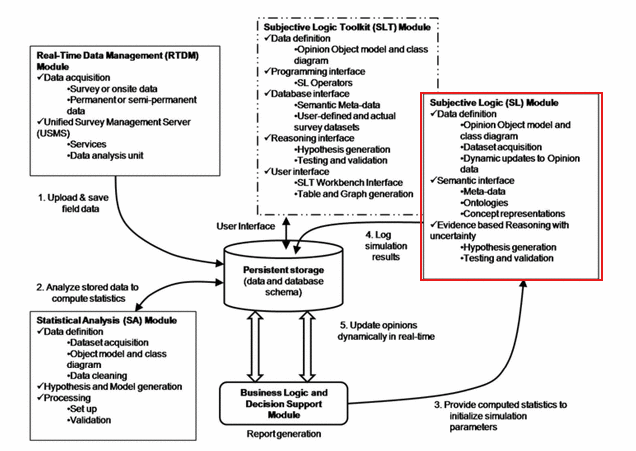
\includegraphics[width=\textwidth]{../img/udmdss.jpg}
  \caption{Unified Data Management and Decision Support System (UDMDSS) \cite{kent2010application}}
  \label{fig:udmdss}
\end{figure}







\section{Automated Reasoning}

Automated reasoning is a topic of Artificial Intelligence that has to do with
the construction of systems that can reason with information and draw conclusions.
Wos et al define an automated reasoning program to be one that ``employs an unambiguous
and exacting notation for representing information, precise inference rules for
drawing conclusions, and carefully delineated strategies to control those inference
rules'' \cite{wos1984automated}. Reasoning can either be

\begin{itemize}
  \item \emph{deductive}: where from a set of initial facts and rules of the form ``if X then Y'',
    we can compute the truth or falsity of theorems with absolute certainty through the use of \emph{Modus Ponens} \cite{sternberg2008cognitive}
    For example: suppose we know for absolute certainty that all professors are cranky, and that
    Dr. X is a professor. We therefore must conclude that Dr. X is cranky.
  \item \emph{inductive}: where from some observations we formulate a hypothesis
    and then verify that hypothesis by testing that it holds for new observations. In contrast with deduction, inductive
    conclusions should not be certain, but probable, given the supporting evidence \cite{copi2007essentials}.
    For example, a scientist
    may, after several observations of birds flying, construct the hypothesis that all birds fly.
    The scientist must modify her hypothesis upon observing an ostrich.
  \item \emph{abductive}: where we compute the best possible hypothesis that explains
    some observation \cite{josephson1996abductive}. As an example, physicians must use abductive reasoning every day in their
    work, as all that they can observe are symptoms, not the causes of those symptoms. Therefore
    if there exist several competing explanations as to why the patient has a terrible cough,
    the doctor must abduce the most likely hypothesis, and then test that hypothesis to ensure
    its validity.
\end{itemize}

%
% Discuss certainty vs uncertainty here.
%


%
% Certain vs Uncertain reasoning.
% Certain: closed world. Propositional logic, modal logic, etc.
% Uncertain: open world. Most of the weight of the thesis goes into this section...
%



Unlike deduction, neither induction nor abduction can be used to reason with absolute certainty.
Since the validity of collected population survey data is not absolutely certain (data can be missing or
unclear, the clerk may have entered the survey data into the system incorrectly, or a whole host of
other issues) the focus of this thesis is on the development of a software library that can
reason with uncertain information. As will be shown in Section \ref{sec:subjective-logic-intro},
in the case of Subjective Logic, as the amount of evidence tends toward infinity, the amount of
uncertainty tends to zero, leaving a pure probability.




\section{Uncertain Reasoning}
\label{sec:uncertain-reasoning}


Since the early days of Artificial Intelligence, researchers have been interested in modeling
how humans perform various kinds of reasoning \cite{russell2003}, and more recently (late 1980's to early 1990's)
researchers have developed successful techniques for constructing artificial systems that can reason with
uncertainty \cite{russell2003}. Tools that are used by researchers for handling uncertain or incomplete
information include, but are not limited to

\begin{itemize}
  \item Bayesian Probability
  \item Fuzzy Logic
  \item Dempster-Shafer Theory
  \item and more recently, Subjective Logic
\end{itemize}

In this section we discuss the above mentioned calculi, and in Section \ref{sec:tools-for-reasoning} we discuss
various languages, workbenches, and tools that are available for researchers.


%
% Discuss the ``theory'' here, not the tool. So bayesian probability, fuzzy logic, DS-Theory, SL.
%



\subsection{Bayesian Probability}

Bayesian Probability is an interpretation of the concept of probability that
can be seen an extension of propositional logic \cite{carnap1962logical}. It allows for reasoning with
propositions whose truth values are uncertain. Being an evidential probability,
the prior probability of a proposition (the probability of the proposition being
true prior to any evidence being accounted for) is assigned, and as evidence is
accounted for, the probability of the proposition is updated through a mechanism
called \emph{Bayesian Updating} \cite{paulos2011mathematics}. Unlike a frequentist
view of probability, in which the probability of a proposition represents the frequency
of the event occurring, in Bayesian Probability the probability of a proposition
represents a state of belief \cite{de1977theory}.

Reasoning with Bayesian Probability amounts to the following:

\begin{enumerate}
  \item Represent all sources of uncertainty as statistical random variables \cite{dupre2009new}.
  \item Determine and assign a prior probability distribution to the random variables.
  \item As more evidence is made available, update the probability distributions by applying Bayes' Formula:
\end{enumerate}

$$
P(A | B) = \frac{P(B | A) \times P(A)}{P(B)}
$$

$P(A)$ represents the prior probability of the proposition $A$ being true, and $P(A | B)$
is the conditional probability of $A$ being true given $B$ is true. Therefore, as new evidence becomes
available, the probability distributions describing the propositions are updated, and these
updated probabilities are then used as priors for further calculations with new evidence.

While Bayesian Probability appears to be a fairly simple method of extending propositional
logic to handle uncertainty, one issue that arises is when one wants to carry out
abductive inference. The \emph{base rate fallacy} occurs when one assumes that
$P(A | B) = P(B | A)$ \cite{koehler1996base}, and therefore when one wants to reason backwards from
some observable evidence to the likely hypothesis, the conditional probabilities must
first be inverted \cite{josanginverting}. Subjective Logic, as will be shown, supports both deductive and
abductive reasoning as operators, and thus no confusion can occur so long as the correct
operator is chosen.





\subsection{Fuzzy Logic}

Fuzzy Logic is a many-valued logic that supports reasoning with approximate
truth values, rather than exact truths as in classical logic \cite{perfilieva1999mathematical}.
The term ``fuzzy logic'' was first introduced by Zadeh \cite{zadeh1965fuzzy} in his description
of \emph{Fuzzy Set Theory}, and since then it has been applied to fields such as
Control Theory, Automated Reasoning, and Machine Learning \cite{bansod2005soft}.

Given a predicate $P$ and a variable $x$, let $P(x)$ be a function that maps
$x$ to a value on the interval $[0, 1]$. This function represents the degree of which
$x$ satisfies $P$. For example, consider two predicates $Red$ and $Yellow$. Given
the variable $orange$ representing the colour orange, one observer might say that
$Red(orange) = 0.4$, and that $Yellow(orange) = 0.8$. That is, the colour orange
is more ``yellow'' than it is ``red''. However a different observer might assign
a different degree of membership to the colour.

Fuzzy Logic supports the operators AND and OR, just like in classical logic, but since
the degrees of truth are continuous values between 0 and 1, a simple truth-table will
not suffice for representing the logical operators. Therefore, Fuzzy Logic defines
x AND y to be the minimum value of the two degrees of truth, and x OR y to be the
maximum value. The negation of a degree of truth is 1 minus the degree.

Fuzzy Logic has been suggested as a method of handling uncertainty in the design
of expert systems by Zadeh \cite{zadeh1983role}. In fact, Zadeh claims that
Fuzzy Logic subsumes both Probability Theory and Predicate Logic and allows for
uncertainty to be handled in one single conceptual framework. It is claimed, however,
by Russell and Norvig in their popular textbook \emph{Artificial Intelligence: A Modern Approach}
\cite{russell2003} that Fuzzy Logic is not a method of uncertain reasoning at all,
because it simply replaces crisp truth values with approximate ones. Therefore, they
claim that Fuzzy Logic is a method of representing vagueness, not uncertainty.



\subsection{Dempster-Shafer Theory}
\label{sec:dst}

Dempster-Shafer Theory is a mathematical and philosophical theory of evidence
\cite{shafer1976mathematical}. It is an extension of Bayesian Probability in which
probabilities are assigned not to individual random variables, but to sets of them.
The belief of an individual random variable is bounded above and below by two values:
the \emph{plausibility} of the random variable, and the \emph{belief} of it.

Given a \emph{frame of discernment}, a set containing all mutually exclusive atomic
events that are of interest to our reasoning system, one constructs a \emph{basic belief assignment},
or BBA, which assigns a measure of belief between zero and one to subsets of the frame. BBA's are additive: if
$X$ is a frame of discernment and $m$ is a BBA over $X$, then $\sum_{x \subset X} m(x) = 1$.
Furthermore, no mass is assigned to the empty set: $m(\emptyset) = 0$.

Given a BBA $m$ over a frame $X$, one can compute the belief and plausibility of a subset
$A$ of $X$ by the following expressions:

\begin{itemize}
  \item $bel(A) = \sum_{B \subseteq A} m(B)$
  \item $pl(A) = 1 - bel(\overline{A})$
\end{itemize}

These two values bound the probability of $A$ from below and above. That is,
$bel(A) \leq P(A) \leq pl(A)$. The real novelty of Dempster-Shafer Theory, however, is
\emph{Dempster's Rule of Combination}, which states how two BBA's generated
by two observations can be combined together \cite{dempster1968generalization}. Let $m_1$ and $m_2$ be two BBA's over a
frame of discernment $X$. We combine together the two BBA's by computing what is referred to
as the \emph{joint mass}, denoted as $m_{1,2}$, by the following equation:

\begin{equation*}
  \begin{split}
    m_{1,2}\left(\emptyset\right) & = 0 \\
    m_{1,2}\left(A\right)         & = \left( m_1 \otimes m_2\right) = \frac{1}{1 - K} \sum_{B \cap C = A \neq \emptyset} m_1(B) m_2(C)
  \end{split}
\end{equation*}

$K$, which represents the amount of conflicting belief between $m_1$ and $m_2$, is $\sum_{B \cap C = \emptyset} m_1(B) m_2(C)$.

While fairly straight forward to calculate, it has been shown by Zadeh \cite{zadeh1979validity, zadeh1986simple}
that Dempster's Rule generates counter-intuitive results when there is a high degree of
conflict between the two belief masses, and Josang and Pope claimed that Dempster's Rule actually
represents a method of preference combination while serving as an approximation for other forms of belief
combination such as the cumulative or average fusion of two beliefs \cite{josang2012dempster}. Subjective Logic, which we introduce next,
contains several operators for combining beliefs together \cite{josang2012interpretation, josang2010cumulative, josang2009fission, josang2009cumulative},
that serve as better tools for combining evidence from different sources in different scenarios.
Furthermore, Judea Peal has claimed that it is misleading to interpret belief functions as anything
other than the probability that a given proposition is provable from a set of other
propositions that have assigned probabilities \cite{pearl1988probabilistic, pearl1988probability, pearl1990reasoning}.

Despite these criticisms, Dempster-Shafer Theory has seen much success when applied to
problems such as sensor fusion \cite{wu2002sensor, murphy1998dempster, basir2007engine} and
neural network classification \cite{denoeux2000neural, rogova1994combining}.




\subsection{Subjective Logic}
\label{sec:subjective-logic-intro}

Subjective Logic was introduced by Audun Josang \cite{josang2001logic} as an
extension to probabilistic logic that fixes some of the issues with
Dempster-Shafer Theory \cite{josang2012dempster} that have been mentioned in Section \ref{sec:dst}.
Though it is relatively young and is under constant refinement,
Subjective Logic has been shown to be effective
across a range of areas that require uncertain reasoning, such as
trust network analysis \cite{josang2006trust, josang2008optimal},
modeling trust on mobile ad-hoc networks \cite{li2004trust, liu2011novel},
and arguing with evidence \cite{oren2007subjective, josang2000legal}.






\subsubsection{Subjective Opinions}

The primary building blocks of Subjective Logic expressions are
objects called \emph{subjective opinions} \cite{josang2001logic}. Given a frame of discernment $\Theta$, a subjective
opinion over $\Theta$ is a 3-tuple consisting of the following elements:

\begin{itemize}
  \item A \emph{belief vector}, $b_\Theta$, of assigned belief mass that spans the \emph{reduced power set}
    of $\Theta$. The reduced power set is defined as $R \left(\Theta\right) = 2^\Theta \setminus \lbrace \Theta, \emptyset \rbrace$.
  \item A scalar, $u_\Theta$, that represents the unassigned belief mass
    $u_\Theta + \sum_{x \in R\left(\Theta\right)} b_\Theta\left(x\right) = 1$
  \item A vector of prior belief, $a_\Theta$, that spans the frame $\Theta$
\end{itemize}

such that the following conditions hold:

\begin{enumerate}
  \item $\forall x \in R\left(\Theta\right), b_\Theta\left(x\right) \in \lbrack 0, 1\rbrack$
  \item $\forall x \in \Theta, a_\Theta\left(x\right) \in \lbrack 0, 1\rbrack$
  \item $u_\Theta \in \lbrack 0, 1\rbrack$
  \item $u_\Theta + \sum_{x \in R\left(\Theta\right)} b_\Theta\left(x\right) = 1$
  \item $\sum_{x \in \Theta} a_\Theta\left(x\right) = 1$
\end{enumerate}

Opinions are written as $\omega^A_\Theta = \langle b^A_\Theta, u^A_\Theta, a^A_\Theta \rangle$, where
$A$ is the (optional) agent who owns that particular belief.

Elements of $R\left(\Theta\right)$ such that $b_\Theta\left(x\right) > 0$ are called \emph{focal elements}.
Subjective opinions where the focal elements are all singleton sets - that is, every focal element is
simply an element of $\Theta$ - are referred to as \emph{multinomial opinions}. Multinomial opinions
defined over frames of cardinality 2 are referred to as \emph{binomial opinions}. The most general of
opinions, subjective opinions, are also referred to as \emph{hyper opinions}. Lastly, opinions can either
be \emph{dogmatic}, when $u_\Theta$ is zero, or \emph{uncertain} otherwise. The six classes of subjective
opinions are summarized in Table \ref{tbl:sl-opinions}.

\begin{table}
  \begin{center}
    \begin{tabular}{ r|c|c|c| }
      \multicolumn{1}{r}{}
      &  \multicolumn{1}{c}{$|\Theta| = 2$}
      &  \multicolumn{1}{c}{$|\Theta| > 2$}
      &  \multicolumn{1}{c}{$|R(\Theta)| = 2^{|\Theta|} - 2$} \\
      \cline{2-4}
      $u > 0$ & Uncertain Binomial & Uncertain Multinomial & Uncertain Hyper \\
      \cline{2-4}
      $u = 0$ & Dogmatic Binomial & Dogmatic Multinomial & Dogmatic Hyper \\
      \cline{2-4}
    \end{tabular}
  \end{center}

  \caption{Subjective Logic Opinions}
  \label{tbl:sl-opinions}
\end{table}

Binomial opinions have a special notation that is used to emphasize the binary nature of the frame of
discernment \cite{josang2001logic}. Given a frame $\Theta = \lbrace x, \lnot x \rbrace$, the binomial opinion of $x$ is written
as $\omega_x = \langle b_x, d_x, u_x, a_x \rangle$, where

\begin{itemize}
  \item $b_x$ is the belief of event $x$ being true.
  \item $d_x$ is the belief of event $x$ being false.
  \item $u_x$ is the uncertainty of whether $x$ is true or false.
  \item $a_x$ is the belief of $x$ being true prior to the collection of evidence.
\end{itemize}

Opinions in Subjective Logic can be mapped to and from probability density functions from Probability
Theory \cite{josang2001logic, josang2012interpretation}. Binomial opinions correspond to \emph{beta probability density functions} (PDFs),
multinomial opinions correspond to \emph{dirichlet PDFs}, and hyper opinions correspond
to \emph{hyper-dirichlet PDFs}. For evidence-based reasoning this is a boon because the
Beta PDF acts as a \emph{conjugate prior} to the binomial distribution, and
the Dirichlet PDF is prior to the multinomial \cite{schlaifer1961applied}. This means that through the mapping,
subjective opinions can be used anywhere one could use Bayesian Inference, where the Bayesian Update
mechanism updates the opinions to take into account new evidence.




\subsubsection{Subjective Logic Operators}

Subjective Logic includes a wealth of operators for working with all classes of opinions. It includes
the traditional binary logic operators such as \emph{and}, \emph{or}, and \emph{not}, which are
upgraded to incorporate uncertainty, as well as the set-theoretic operators \emph{union} and
\emph{set-difference}. In the case of absolute belief ($b_x = 1$) or disbelief ($d_x =1$), these
binomial operators behave the same as they would in traditional logic \cite{mcanally2004addition, josang2005multiplication}.

Subjective logic also includes operators for working with multinomial opinions, such as
cumulative and averaging \emph{fusion} and \emph{unfusion} \cite{josang2010cumulative, josang2009cumulative, josang2009fission, josang2012interpretation}.
These operators allow for combining
multinomial opinions from different sources. Subjective Logic also includes operators for performing
transitive trust analysis \cite{josang2001logic, josang2006trust}, where an agent A has an opinion of agent B, and agent B has an opinion of
the event X. Agent A, through its opinion of agent B, can derive an opinion of event X by using one
of several \emph{discounting} operators. Subjective Logic also includes an operator for
\emph{belief constraining} \cite{josang2012dempster}, which can be used when multiple agents need to reach a consensus opinion.
This operator is in fact equivalent in meaning to Dempster's rule of combination \cite{josang2012dempster}.

Lastly, Subjective Logic also includes operators for performing uncertain reasoning \cite{josanginverting, josang2008conditional, josang2008abductive}.
It includes \emph{deduction} and \emph{abduction} operators for subjective opinions, thereby allowing Subjective
Logic to be used for intelligence analysis \cite{pope2005analysis},
bayesian network analysis \cite{josang2008conditional}, and other actions that
require reasoning when uncertainty is present.




\section{Languages and Tools for Automated Reasoning}
\label{sec:tools-for-reasoning}

In Section \ref{sec:uncertain-reasoning} we introduced various systems for automated reasoning. In this
section we discuss some languages and tools that have been developed for the previously mentioned
systems. Note however that as far as we know, there do not exist any languages or tools for working
with Subjective Logic.





\subsection{Weka}

\emph{Waikato Environment for Knowledge Analysis (WEKA)} is a popular workbench for machine learning
\cite{witten2005data}. It contains many popular algorithms and visualization techniques for performing data mining,
data analysis, and predictive modeling. It is developed in the JAVA programming language, and is
distributed as \emph{Free Software} under the GNU General Public License.

Though freely available, Weka requires all data to be described using a fixed number of attributes and all
data must be stored in a single file or relational table \cite{reutemann2005toolbox}. There exist tools however for converting data into
the format required for Weka \cite{reutemann2005toolbox}.





\subsection{DSI Toolbox}

\emph{Dempster-Shafer with Intervals (DSI)} is a verified MATLAB toolbox
for computing with Dempster-Shafer Theory \cite{auer2010verified}. The authors
claim that DSI introduces intervals to a previously developed IPP toolbox \cite{limbourg2007}, and that because of this
modification they claim that DSI does not suffer from the same rounding errors that occur in IPP.
We follow a similar approach in the design of our library: in order to avoid the possibility of rounding errors in Subjective Logic,
we represent each numeric value as a rational number. As will be explained in Section \ref{sec:limitations},
this representation may not always be desirable, as it removes the ability for prior beliefs to be populated
with irrational numbers such as $\frac{1}{e}$.



%\subsection{Repast}





\subsection{R}

R is a programming language and interactive environment for statistical computing \cite{team2012r}.
It is popular among statisticians and data miners \cite{fox2005using, vance2009data}, and is a powerful
and free alternative to other non-free statistical tools
such as SAS \cite{delwiche2012little} and SPSS \cite{quintero2013workload}. R can be extended through
user-defined packages, many of which are available through repositories such as the \emph{Comprehensive R Archive Network (CRAN)}
and \emph{Bioconductor}, a project which focuses on the analysis of genomic data in molecular biology.

Though powerful, we believe the language is best suited for designing statistical software, not general purpose
programming. For the development of our library for Subjective Logic, we chose to use the Haskell
language over R, as we feel that Haskell has better support for everyday programming.





\subsection{Prolog}

\emph{Prolog} is a Logic Programming Language, which means that every computation must be
expressed as a logical statement \cite{sterling1994art}. Despite this seemingly strange restriction, Prolog is
a general-purpose programming language \cite{sterling1994art}.

As mentioned, all computations in Prolog are expressed as logical statements. In particular,
expressions in Prolog are \emph{Horn Clauses}: logical expressions of the form

$$
head :- X1, X2, ... XN
$$

meaning the statement $head$ is true only when statements $X1$ through $XN$ are also true \cite{horn1951sentences}.
As an example of how one can represent computations in Prolog, the following program computes
the factorial of a number:

\begin{code}
factorial(0, X) :- X = 1.
factorial(N, X) :- NN = N - 1, factorial(NN, X1), X = X1 * N.
\end{code}

It was the language of choice for Japan's ambitious fifth generation computing project \cite{shapiro1983fifth},
and Prolog still sees much use in the Natural Language Processing community
\cite{covington1994natural, pelletier2006representation},
as it has excellent support for implementing \emph{definite-clause grammars} \cite{pereira1980definite}.
Prolog, however, does not have built-in support for uncertainty. Because it is a general purpose
programming language, one could theoretically construct an automated reasoning program in Prolog that
does handle uncertainty, however it would fight against the spirit of the language.








%
% TODO: Add a section on agent-based modelling.
%



\begin{table}
  \begin{center}
    \begin{tabularx}{\textwidth}{| l | l | l | X |}
      \hline
      Name & Method of Reasoning & Data Representation & Notes \\
      \hline
      Prolog                & Deduction                   & Horn Clauses & Unideal for uncertainty. All computations represented as logical deductions. \\
      \hline
      R                     & Bayesian Statistics         & Data tables  & Powerful for statistical computation.                                         \\
      \hline
      Weka                  & Machine learning algorithms & Data tables  & Vast array of tools. Data must conform to a certain format to be usable.     \\
      \hline
      DSI                   & Dempster-Shafer Theory      & Beliefs      & MATLAB workbench. Uses intervals instead of floating point math.             \\
 %     Repast                & Agent-based models          & Priors               \\
      \hline
    \end{tabularx}
  \end{center}

  \caption{Summary of Discussed Reasoning Tools}
  \label{tbl:reasoning-tools}
\end{table}





%
% TODO: Add a table of each toolkit / language discussed. Rows:
% 1. Tool name
% 2. Fundamental item for reasoning
% 3. Input Data
% 4. Drawbacks.
%









\subsection{Summary}

There currently exist many tools for developing automated reasoning systems, and we have summarized a few
of them in the previous section and in Table \ref{tbl:reasoning-tools}.
Due to it being quite young in comparison to other systems, there do not yet exist any
comprehensive tools for developing applications with Subjective Logic. In the next section
we present an overview of the Haskell programming language, our implementation language for a new Subjective Logic
library, and in Chapter \ref{chap:sl-in-haskell} we present SLHS: Subjective Logic in Haskell.






\section{Functional Programming in Haskell}

\emph{Haskell} is a strongly typed, non-strict, pure functional
programming language \cite{hudak1992report} which was initially
developed to be a common language for researchers interested in
non-strict, pure functional programming languages
\cite{hudak2007history}.
By \emph{non-strict}, we mean that Haskell
evaluates expressions in a \emph{call-by-need} manner: expressions are
only evaluated if and when they are required \cite{henderson1976lazy}. Haskell is a
\emph{functional programming language}, where the meaning of
\emph{functional} is the style of programs as described by John Backus
in his Turing award lecture: \emph{Can Programming Be Liberated from
  the von Neumann Style?}\cite{backus1978can}.  Lastly, Haskell is
\emph{pure} in the sense that all functions are functions in the
mathematical sense: they depend only on their inputs to produce their
outputs. Haskell does not support the use of global state when
writing programs.

In this section we will briefly describe the syntax of Haskell in
order to give the reader enough familiarity to understand the code
listings of Chapter \ref{chap:sl-in-haskell}. This section is by no
means exhaustive in its treatment of Haskell. For readers who wish to
learn Haskell in more depth, we suggest the book \emph{Real World Haskell} \cite{o2008real}.

Functions in Haskell are written as equations, with parameters separated
by white space. For example, the function to compute factorials can be
written as

\begin{spec}
factorial 0 = 1
factorial n = n * factorial (n - 1)
\end{spec}

All expressions in Haskell have \emph{types}. For example, the type of the literal
5 is \emph{Int}. Syntactically this is expressed as \emph{5 :: Int}. The function
\emph{factorial} above has the type \emph{Int $\rightarrow$ Int}.

Lists in Haskell are enclosed in square braces, and their elements must be of all
the same type. As an example, the following is a valid list:

\begin{spec}
names :: [String]
names = [''John'', ''Paul'', ''George'', ''Ringo'']
\end{spec}

whereas the following is invalid:

\begin{spec}
things = [5, ''seven'', 2/3]
\end{spec}

Types in Haskell can be organized into \emph{Type Classes}, where each type in a
type class must have certain required operations defined over it. For example, consider
the following class:

\begin{spec}
class Monoid n where
    id  :: n
    (<>) :: n -> n -> n
\end{spec}

which states that a type $n$ satisfies the properties of being a \emph{Monoid} if there exists
a element $id$ of type $n$, and there exists an operator for combining elements of type $n$.
Unfortunately the additional requirement of associativity cannot be expressed in Haskell.
Instances of the Monoid class can then be defined for individual types:

\begin{spec}
instance Monoid Int where
    id = 0
    x <> y = x + y
\end{spec}

One type class in particular gets special attention in Haskell. Types that are instances of
class \emph{Monad} are very popular in functional programming, and Haskell in particular \cite{peyton1993imperative}. Monads
are mathematical objects from \emph{category theory} that are prevalent throughout Haskell.
They were first introduced by Eugenio Moggi \cite{moggi1991notions} and have subsequently been
used for parsing \cite{hutton1998monadic, leijen2001parsec, hafiz2010lazy}, modeling state
\cite{launchbury1994lazy}, and much more. Most
importantly, Haskell uses monads to handle input/output \cite{peyton1993imperative}, which allows Haskell to read
input from the user, and send output to the computer screen, while remaining a pure functional
language. Types that are instances of \emph{Monad} require two operations to be present:

\begin{spec}
class Monad m where
    return :: a -> m a
    (>>=)  :: m a -> (a -> m b) -> m b
\end{spec}

The first function, \emph{return}, injects an object of type $a$ into an object of type $m\,a$, where
$m$ is some monad. The second operator takes in an object of type $m\,a$ on the left hand side, and
a function $f$ from $a$ to $m\,b$ on the right hand side, and returns an object of type $m\,b$.
Informally, the operator unwraps the object of type $a$ from the object of type $m a$, and then applies
the function to it to obtain a result.






\section{Summary}

In this chapter we discussed the key ideas of decision support
systems, followed by an overview of automated reasoning, and an
introduction to various uncertain reasoning systems. We then introduced Subjective
Logic and presented a brief overview of the Haskell programming
language. In the next chapter we present our thesis problem,
our thesis hypothesis, our research objectives, and our methodology.


\end{document}
